\documentclass{article}
\usepackage[paperwidth=8.5cm, paperheight=5cm, margin=0in]{geometry}
\usepackage{tikz}
\usetikzlibrary{calc,patterns,decorations.pathmorphing,decorations.markings}
\usetikzlibrary{arrows}


\newcommand{\masswidth}{.8cm}
\newcommand{\massheight}{0.6cm}
\newcommand{\wallthickness}{0.25cm}
\newcommand{\figwidth}{4.1cm}
\newcommand{\springlength}{\figwidth-2*\wallthickness-3*\masswidth}
\newcommand{\halfspringlength}{\figwidth/2-\wallthickness-3*\masswidth/2}
\newcommand{\onepointfivespr}{1.5*\figwidth-1.5*2*\wallthickness-1.5*3*\masswidth}
%\newcommand{\springlength}{1.5cm}
\newcommand{\leftwalleastpos}{0}
%\newcommand{\leftwalleastpos}{-{3cm}}
\newcommand{\massonepos}{\springlength+\masswidth/2}
\newcommand{\masstwopos}{\massonepos+\masswidth+\springlength}
\newcommand{\massthreepos}{\masstwopos+\springlength+\masswidth}
\newcommand{\rightwallpos}{\massthreepos+\springlength+\masswidth/2}
\newcommand{\konepos}{\halfspringlength}
\newcommand{\konetwopos}{\massonepos+\halfspringlength+\masswidth/2}
% \newcommand{\ktwothreepos}{\masstwopos+\masswidth/2+\halfspringlength}
\newcommand{\ktwothreepos}{\masstwopos}
\newcommand{\kthreepos}{\massthreepos+\halfspringlength+\masswidth/2}
\newcommand{\spronethreey}{1.2cm}  % height of spring k13
\newcommand{\lowerlevel}{-1.6cm}
\newcommand{\ktwopos}{\springlength+2*\masswidth/3}
\newcommand{\konethreex}{\massonepos+\onepointfivespr+1.5*\masswidth}
\newcommand{\wally}{-.8cm}
\newcommand{\labelheight}{-.9cm} %+.76cm
\newcommand{\wallheight}{2.8cm}

\begin{document}



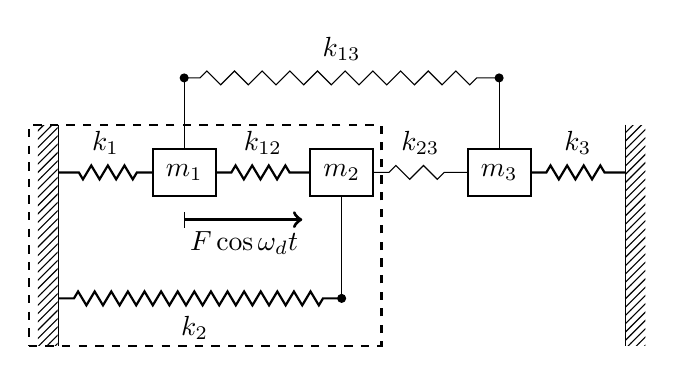
\begin{tikzpicture}[]
\tikzstyle{spring}=[thick,decorate,decoration={zigzag,pre length=0.2cm,post length=0.2cm,segment length=6}]
\tikzstyle{weakspring}=[decorate,decoration={zigzag,pre length=0.2cm,post length=0.2cm,segment length=10}]
\tikzstyle{wall}=[fill,pattern=north east lines,draw=none,minimum width=\wallthickness,minimum height=\wallheight]

%% draw walls
\node (leftwall)  [wall, xshift=\leftwalleastpos, yshift=\wally,anchor=east] {};
\draw (leftwall.north east) -- (leftwall.south east);
\node(rightwall)[wall, xshift =\rightwallpos,yshift=\wally,anchor=west]{};
\draw (rightwall.north west) -- (rightwall.south west);

%% three masses
\node(M1)  [minimum width=\masswidth,minimum height=\massheight, xshift=\massonepos, style={draw,outer sep=0pt,thick}] {$m_1$};
\node(M2)  [minimum width=\masswidth,minimum height=\massheight, xshift =\masstwopos,style={draw,outer sep=0pt,thick}] {$m_2$};
\node(M3)  [minimum width=\masswidth,minimum height=\massheight, xshift =\massthreepos,style={draw,outer sep=0pt,thick}] {$m_3$};

%% dotted box
\node(dottedbox) [minimum width=\masstwopos-\leftwalleastpos+\masswidth*1.1, 
			   minimum height=\wallheight, 
			   xshift=\massonepos+\masswidth/3, 
			   yshift=\labelheight+.1cm,
			   style={draw, outer sep=0pt, dashed, thick}]{};

%% four main springs
\draw [spring] (M1.west)  -- (\leftwalleastpos,0);
\node [above] at (\konepos,.1cm) {$k_1$};
\draw[spring](M1.east)--(M2.west);
\node [above] at (\konetwopos,.1cm) {$k_{12}$};
\draw[weakspring](M2.east)--(M3.west);
\node[above] at (\konethreex,.1cm) {$k_{23}$};
\draw[spring](M3.east)--(\rightwallpos,0);
\node [above] at (\kthreepos,.1cm) {$k_{3}$};

%% spring 2
\draw [fill] circle [radius=.05cm, xshift=\masstwopos, yshift=\lowerlevel] {};  % xshift to match m2
\draw (M2.south)--(\masstwopos,\lowerlevel);
\draw[spring] (\leftwalleastpos, \lowerlevel) -- (\masstwopos, \lowerlevel);
\node[below] at (\ktwopos,\lowerlevel-.1cm) {$k_2$};

%% spring 13
\draw [fill] circle [radius=.05cm, xshift=\massonepos, yshift=\spronethreey] {};  % xshift to match m1
\draw(M1.north)--(\massonepos,\spronethreey);
\draw [fill] circle [radius=.05cm, xshift=\massthreepos, yshift=\spronethreey] {};  % xshift to match m3
\draw(M3.north)--(\massthreepos,\spronethreey);
\draw[weakspring] (\massonepos,\spronethreey) -- (\massthreepos,\spronethreey);
\node [above] at (\ktwothreepos,\spronethreey+.1cm) {$k_{13}$};

%% force label
\newcommand{\arrowheight}{\labelheight+.3cm}
\newcommand{\Fcosheight}{\labelheight} % + .27 cm
\node[ anchor=west] at (\massonepos - .05 cm,\Fcosheight) {$F \cos \omega_d t$};
\draw[very thick,->](\massonepos,\arrowheight) --(1.5cm+\massonepos,\arrowheight);
%\draw (M1.north)--(\massonepos, 1 cm); % option 1
\draw (\massonepos, \arrowheight - .1cm)--(\massonepos, \arrowheight+.1cm); % option 2


%\draw [spring] (leftwall.east) -- (leftwall.east+1cm){k1};

\end{tikzpicture}


\end{document}